\chapter{Introducción}
\label{sec:introduccion}

% Estilo de párrafo de los capítulos
\setlength{\parskip}{0.75em}
\renewcommand{\baselinestretch}{1.25}
% Interlineado simple
\spacing{1}
% Numeración contenido
\pagenumbering{arabic}
\setcounter{page}{1}

La presente sección tiene como objetivo realizar una contextualización del proyecto, analizando la motivación de su existencia, la necesidad que pretende resolver y, por último, introducir el formato y la división en epígrafes de las sucesivas secciones del presente documento.

\section{Motivación y contexto}
Los últimos cincuenta años han supuesto una gran revolución en el área de la informática a nivel mundial ---y, particularmente, nacional---, ejecutándose un proceso de gran expansión y crecimiento del acceso de la sociedad a las nuevas tecnologías, de modo que en la actualidad están presentes en la práctica totalidad de los hogares y puestos de trabajo de España.
Según el Instituto Nacional de Estadística, el 93,9\% de la población española de entre 16 y 74 años ha realizado un uso frecuente de Internet durante el año 2021; porcentaje que crece hasta el 99,8\% ---la práctica totalidad--- al poner el foco en la franja etaria comprendida entre los 16 y los 24 años \cite{INEMyH2021}.

Este pujante crecimiento de la tecnología y su incorporación a la cotidianidad de las personas ha conducido a la introducción de la disciplina de la programación informática en los currículos educativos de múltiples países del primer mundo, entre ellos España. La Ley Orgánica de Modificación de la Ley Orgánica de Educación (LOMLOE) ---actual ley en vigor para la configuración de los pilares esenciales de la educación obligatoria y no universitaria a nivel nacional--- estipula que el ``uso seguro, saludable, sostenible, crítico y responsable de las tecnologías digitales para el aprendizaje, para el trabajo y para la participación en la sociedad'' \cite{BOEMEFP2022} es un ingrediente fundamental en la formación de los más jóvenes, impulsando la educación digital desde las primeras etapas formativas.

Buena muestra de la relevancia que la informática toma en la educación actualmente se aprecia, por ejemplo, en la Comunidad de Madrid, donde se imparte una asignatura llamada ``Tecnología, Programación y Robótica'' en la etapa de Educación Secundaria Obligatoria. Esto hace que todos los estudiantes madrileños de entre 12 y 15 años ---entre los cursos primero y tercero de la citada etapa--- dediquen dos horas lectivas semanales al aprendizaje de destrezas como: la capacidad para crear programas en algún lenguaje de programación textual, el desarrollo de aplicaciones móviles mediante programación por bloques o la creación de páginas web haciendo uso de los gestores de contenidos más extendidos, tal como queda recogido en el currículo establecido para la mencionada materia \cite{CMEdu2015}; entre otras habilidades fundamentales, tales como el uso responsable de la tecnología y las redes sociales o la formación en prevención de riesgos de seguridad informática a nivel de usuario.

Cabe introducir en este punto, además, una especial mención a la situación generada por la COVID-19 a partir de marzo de 2020, que provocó el mayor confinamiento de la sociedad que se recuerda en varias generaciones. Este radical, espontáneo e inesperado cambio del paradigma sociocultural llegó en un punto de digitalización que permitió redirigir el modelo de funcionamiento habitual de la sociedad española hacia un modelo en línea basado en comunicaciones a través de medios digitales en el que las videoconferencias tomaron un papel preponderante. En esta situación, la ciudadanía comenzó a percibir este formato como una alternativa real posible que, si bien puede resultar ``incompleta'' para algunas personas y que no es posible trasladar a algunos sectores laborales y sociales, permite resolver con eficacia las necesidades comunicativas en situaciones en las que no es posible realizar encuentros presenciales.

A este respecto, la \textit{Encuesta de Calidad de Vida} del Instituto Nacional de Estadística recoge en su edición de 2021 \cite{INECOVID_Teletrabajo2020} que, de los cerca de 21 millones de adultos españoles que trabajaron en algún momento durante el año 2020, el 51,1\% no pudieron hacerlo de forma remota porque su puesto de trabajo no estaba correctamente acondicionado o porque sus ocupaciones laborales no podían ser realizadas mediante esta modalidad. Sin embargo, cabe reseñar que el 24,5\% ---algo más de cinco millones de personas--- afirmaron haber teletrabajado a tiempo completo en algún momento durante el año 2020. Esta cifra es significativa en términos relativos, ya que un informe publicado por la misma entidad en febrero de 2020 ---un mes antes del inicio del confinamiento--- \cite{INECOVID_TeletrabajoFeb2020} revela que solo el 4,8\% de los trabajadores empleados en España ejercían su actividad laboral total o parcialmente de forma remota.

Por todo lo anterior, \textit{VSCode4Teaching} es un proyecto que fue concebido e iniciado en el contexto de la incipiente informatización de las aulas, del acceso de los más pequeños de la sociedad a las tecnologías de la información y las comunicaciones ---que toman un papel básico y fundamental en la sociedad actual--- y de la consideración del pensamiento computacional como una competencia básica que permite un desarrollo cognitivo más adecuado a las necesidades del mundo tal como es conocido actualmente. Esta situación sociocultural que dio pie a su creación no solo sigue vigente varios años después, sino que continúa estableciéndose como una realidad pujante y cada vez más aceptada y acogida en la actualidad.

\section{Historia del proyecto \textit{VSCode4Teaching}}
\label{sec:historiaProyecto}
\textit{VSCode4Teaching} es un proyecto que surge con el propósito principal de facilitar la interacción entre el estudiantado y los docentes en el contexto de la impartición de asignaturas o cursos en los que se enseñe cualquier disciplina relacionada con la programación informática. El presente TFG\footnote{TFG. Siglas de ``Trabajo Fin de Grado''.} es el tercer ``capítulo'' de este proyecto, asentándose sobre el resultado de las dos iteraciones anteriores.

El proyecto \textit{VSCode4Teaching} arrancó durante el curso 2019-20, materializándose en el TFG de Iván Chicano Capelo \cite{TFG_Ivan}. Este trabajo dio como resultado la generación de los dos componentes principales que integran la aplicación: el cliente, que es la extensión para Visual Studio Code\footnote{Visual Studio Code. Entorno de desarrollo integrado gratuito divulgado como código abierto que es ampliamente utilizado. Su uso se desarrolla en la \referenciaSeccion{subsec:edicionCodigo}.} que sirve a los usuarios como interfaz para la interacción con el servidor, pudiendo así realizar todos los procesos que permite la aplicación; y el propio servidor, encargado del intercambio de datos con el cliente y con el sistema de persistencia.

En este punto, tras completarse este \textbf{primer hito} de construcción del proyecto, la aplicación cuenta con dos roles o tipos de usuarios: estudiantes y profesores. Específicamente, los docentes disponen de capacidades para la gestión de sus cursos, de los estudiantes inscritos en ellos y de los ejercicios que los conforman, pudiendo crear nuevos ejercicios dentro de los cursos a partir de plantillas disponibles en su sistema de ficheros local. Sobre estos ejercicios, los docentes pueden consultar el estado de ejecución de los ejercicios por parte de los estudiantes descargando sus propuestas de resolución y, además, visualizar el progreso de cada uno en un \textit{dashboard} ---tal como se refleja en la \referenciaFigura{fig:historiaProyecto1Dashboard}---. Además, los profesores pueden compartir un código de cada curso para que los estudiantes se inscriban en él, comparar las propuestas de resolución con la plantilla original a través de una interfaz visual ---como refleja la \referenciaFigura{fig:historiaProyecto1Comparacion}--- e introducir comentarios en los ficheros de las propuestas de los alumnos.

\begin{figure}[h!]
    \centering
    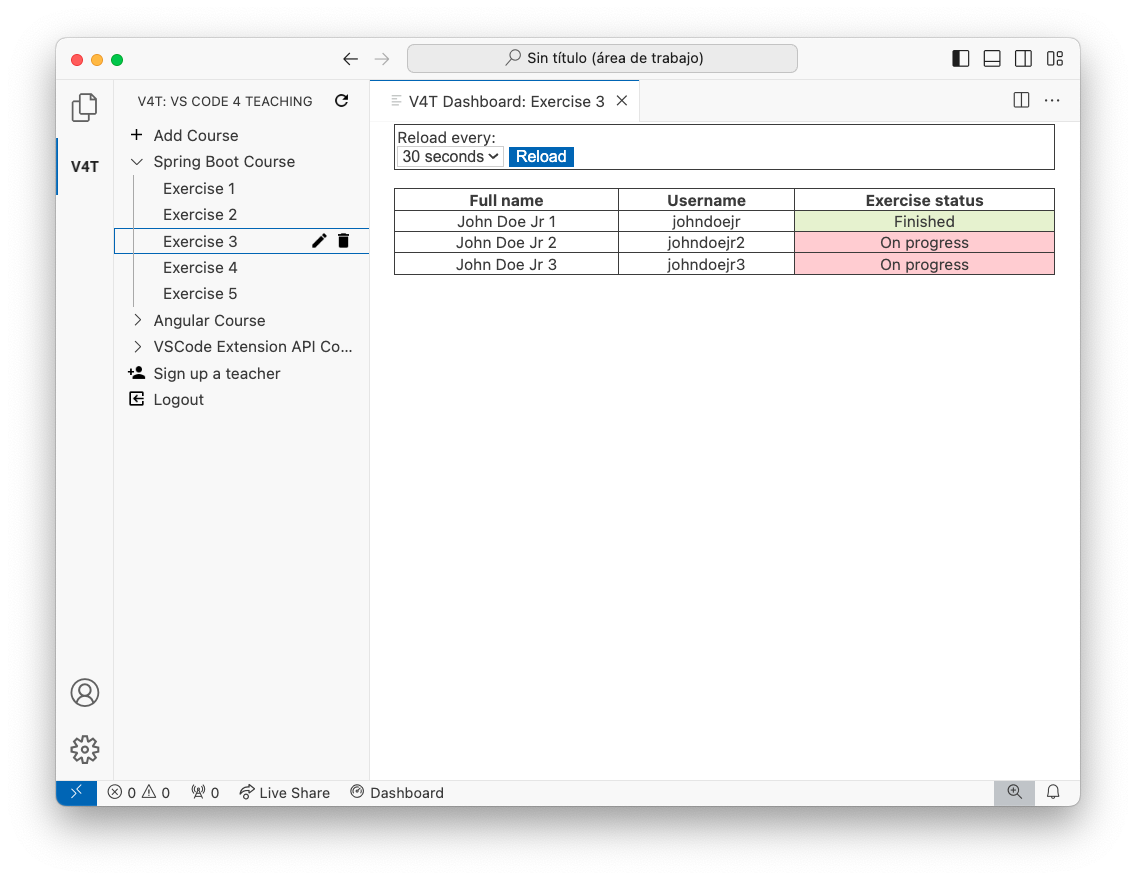
\includegraphics[width=0.825\linewidth]{imagenes/utilizadas/1-introduccion/historia-tfg1-dashboard.png}
    \caption{Captura del \textit{dashboard} para el seguimiento del progreso de los ejercicios en el primer TFG.}
    \label{fig:historiaProyecto1Dashboard}
\end{figure}

\begin{figure}[h!]
    \centering
    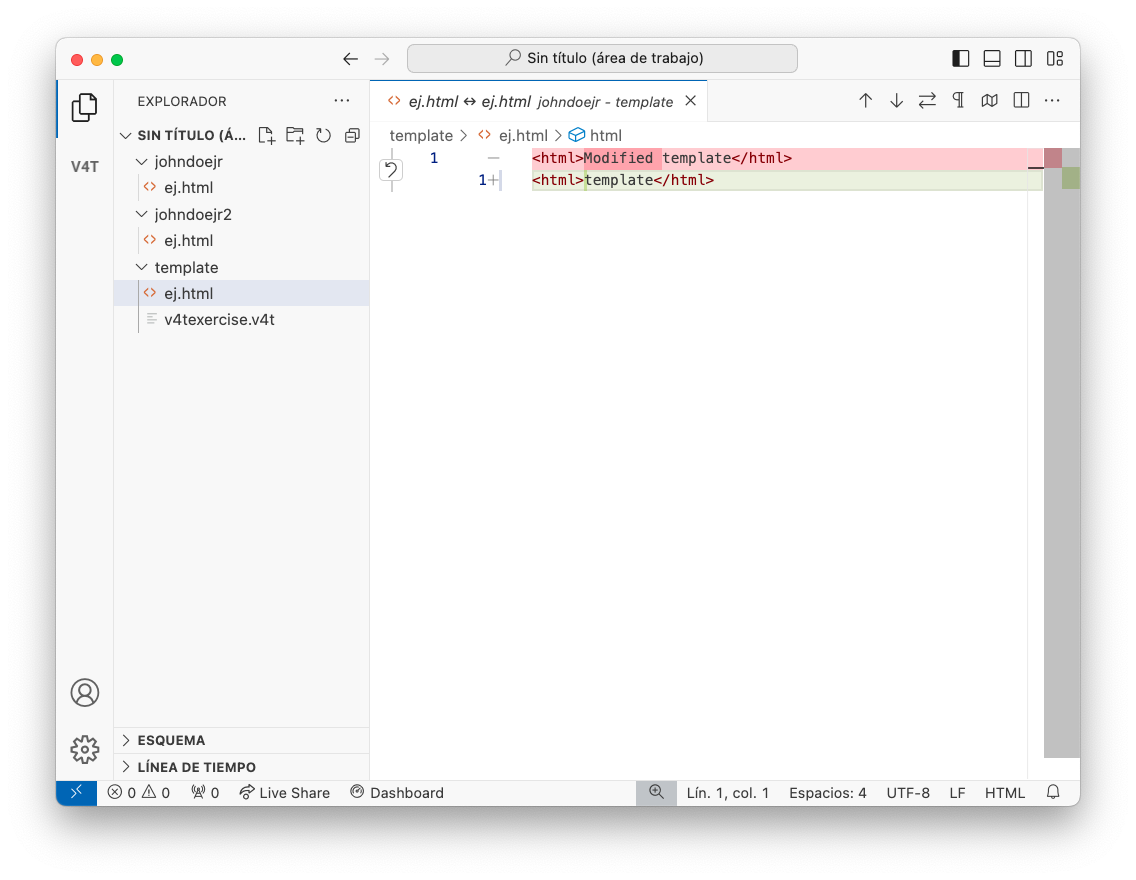
\includegraphics[width=0.825\textwidth]{imagenes/utilizadas/1-introduccion/historia-tfg1-comparacionFicheros.png}
    \caption{Captura de la capacidad para comparación de ficheros en \textit{VSCode4Teaching} en el primer TFG.}
    \label{fig:historiaProyecto1Comparacion}
\end{figure}

Por otro lado, esta primera versión permite a los estudiantes: registrarse en la aplicación, visualizar los cursos en los que están matriculados y sus ejercicios, inscribirse en nuevos cursos utilizando códigos de compartición proporcionados por los profesores, guardar el progreso avanzado durante la realización de los ejercicios y descargar los ejercicios en el punto de progreso en que estuviesen tras la última edición ---o la plantilla en caso de no haberlos comenzado--- y, además, marcar los ejercicios como finalizados para informar al docente, impidiéndose la sincronización de nuevas modificaciones.

Sobre esta base, \textit{VSCode4Teaching} recibió una actualización durante la \textbf{segunda iteración} de su construcción, realizada en el TFG de Álvaro Justo Rivas Alcobendas \cite{TFG_Alvaro}. Durante esta actualización, se buscó potenciar la usabilidad de la herramienta, incorporando numerosas características para, sin modificar reseñablemente el funcionamiento de la aplicación, lograr que todos sus usuarios pudiesen tener una experiencia más completa y mejor informada. Algunas de las mejoras más destacadas son: la incorporación de la actualización en tiempo real del \textit{dashboard} de seguimiento del progreso en la ejecución de ejercicios del que disponen los docentes, que cuenta con mayor cantidad de datos y una apariencia mejorada, tal como se aprecia en la \referenciaFigura{fig:historiaProyecto2Dashboard}; el acceso directo a los ficheros de los estudiantes desde el \textit{dashboard} y la incorporación de una página de ayuda para usuarios ---reflejada en la \referenciaFigura{fig:historiaProyecto2Ayuda}---.

\begin{figure}[ht]
    \centering
    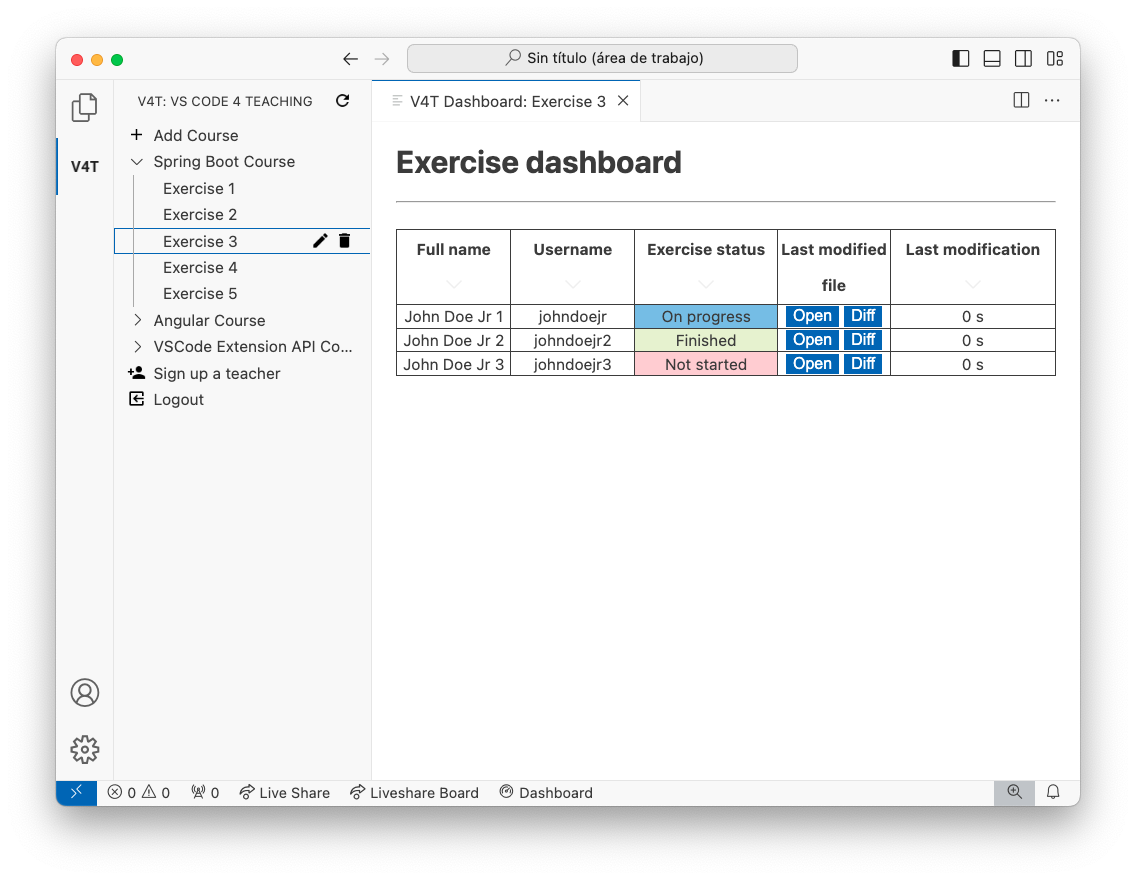
\includegraphics[width=0.825\textwidth]{imagenes/utilizadas/1-introduccion/historia-tfg2-dashboard.png}
    \caption{Captura del \textit{dashboard} para el seguimiento del progreso de los ejercicios en el segundo TFG.}
    \label{fig:historiaProyecto2Dashboard}
\end{figure}

\begin{figure}[ht]
    \centering
    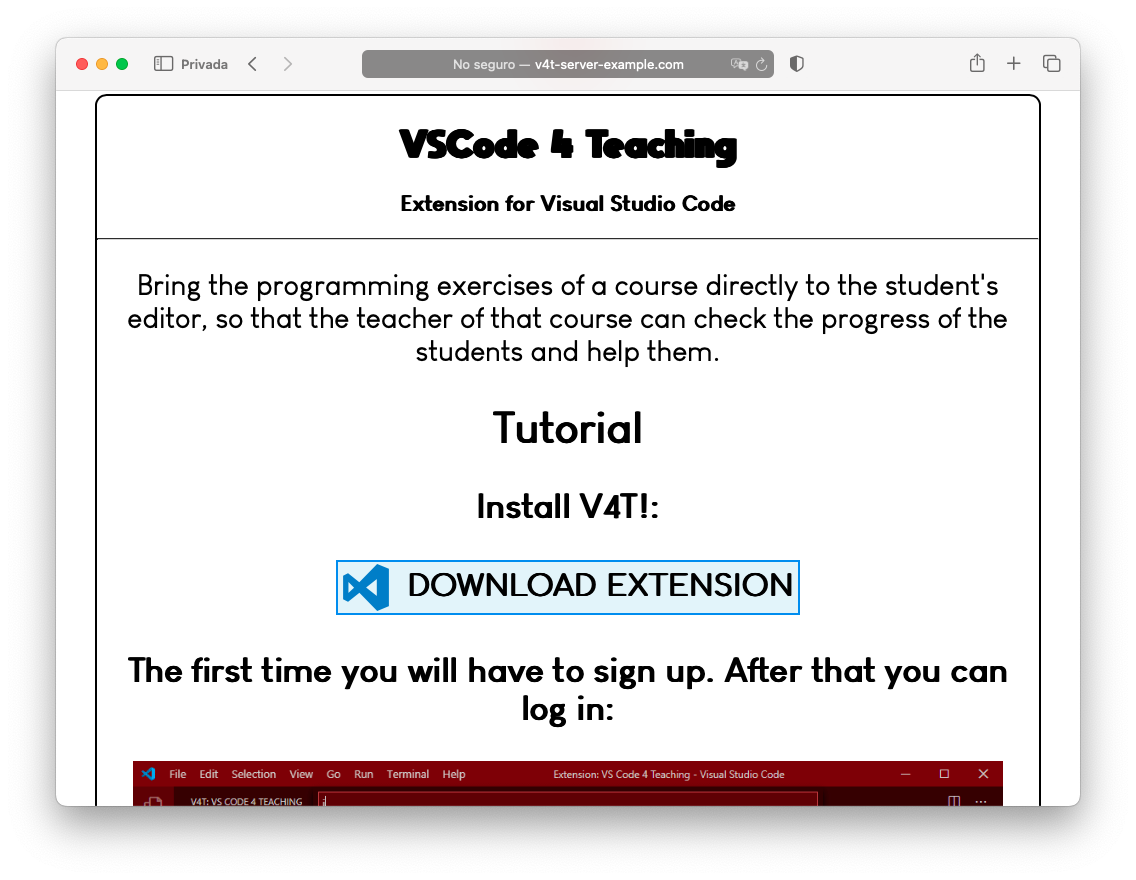
\includegraphics[width=0.825\textwidth]{imagenes/utilizadas/1-introduccion/historia-tfg2-paginaAyuda.png}
    \caption{Captura de la página de ayuda para estudiantes introducida en el segundo TFG.}
    \label{fig:historiaProyecto2Ayuda}
\end{figure}

Una vez explorado el estado inicial del proyecto \textit{VSCode4Teaching} y su funcionalidad disponible, alcanzado mediante las dos evoluciones desarrolladas anteriormente, el presente Trabajo Fin de Grado busca realizar varias tareas enmarcadas esencialmente en el mantenimiento correctivo y perfectivo del proyecto \textit{software} y su funcionalidad, con el fin de alcanzar una tercera evolución de este proyecto para aportarle mayor funcionalidad y calidad. El \referenciaCapitulo{cap:objetivos} detalla el objetivo de este Trabajo Fin de Grado y acota las áreas sobre las que se efectuarán estas mejoras.

\section{Estructura del documento}
El presente documento describe pormenorizadamente cuáles son todas las acciones ejecutadas en materia de evolución y mantenimiento \textit{software} sobre el proyecto en esta tercera iteración de construcción del proyecto \textit{VSCode4Teaching}.

El siguiente apartado (\referenciaCapitulo{cap:objetivos}) recoge los objetivos establecidos en el marco del proyecto que se busca satisfacer en el presente Trabajo Fin de Grado.

El tercer punto (\referenciaCapitulo{cap:tecnolHerramMetodo}) abarca la diversidad de tecnologías y herramientas empleadas para la ejecución del trabajo, así como la metodología de trabajo empleada y la organización para su ejecución.

El apartado cuarto (\referenciaCapitulo{cap:descInformatica}) recoge la descripción informática del trabajo ejecutado. Cabe reseñar que la aplicación queda compuesta por tres grandes componentes: el servidor, la extensión para Visual Studio Code y la aplicación web para navegadores, esta última añadida en el contexto del presente TFG. En torno a cada uno de estos componentes se realiza la descripción de los puntos introducidos en esta sección.

Para finalizar, el capítulo quinto (\referenciaCapitulo{cap:conclusiones}) versa sobre las conclusiones extraídas tras finalizar el desarrollo, analizando la completitud de las necesidades establecidas y estipulando nuevos puntos de mejora para sucesivas iteraciones.

A continuación, una vez finalizado el cuerpo del documento, se introduce la recopilación de referencias bibliográficas a las que aluden las citas introducidas durante el desarrollo del documento.

\noindent\textbf{Nota:} el presente documento contiene diversos enlaces e hipervínculos a páginas web y a otras secciones y epígrafes del documento, destacándolos mediante su introducción en {\color{RedLink}color rojo}. Además, en su edición electrónica, el lector puede hacer \textit{click} sobre estos enlaces para ser conducido al punto al que referencian.
